\chapter{Aktivitätsdiagramm}
\section{Szenario}
Es wird das Szenario eines ersten Tages dualer Studenten im Betrieb beschrieben. Dabei ist geplant, dass etwa 200 Studenten verschiedener Studiengänge anwesend sein werden. Die Studenten sind bereits einzelnen Kursen zugewiesen, welche jeweils einen Ausbilder haben.

Die Studenten werden zunächst freundlich begrüßt und dann in das Audimax gebeten. Dort werden ihnen in verschiedenen Reden die Grundlagen ihrer neuen Tätigkeit erklärt und sie gewinnen erste Eindrücke über das Unternehmen. Im Anschluss daran wird ein Foto der Studenten auf einer angrenzenden Wiese aufgenommen und die Studenten werden in ihre einzelnen Kurse aufgeteilt.

Die Eventplanung ist nur für den ersten Teil des Onboardings verantwortlich. Sobald die Studenten in ihren Kursen ankommen, haben die Ausbilder bereits eigene Aktivitäten geplant. Für das Gruppenfoto und die Reden können Räumlichkeiten des Unternehmens gebucht werden, die Redner werden ebenfalls vom Unternehmen gestellt. Die Eventplanung ist dafür verantwortlich, einen Check-In der Studenten, die technischen Rahmenbedingungen und eine gute Planung zu garantieren.

In diesem Szenario ist das Event bereits mit allen nötigen Informationen geplant und im System angelegt.

\section{Pseudocode}
Der Pseudocode beschreibt hier die Methode \code{EVENT-DURCHFUEHREN}. Aufgrund ihres großen Umfangs, wird sie in mehreren kleineren Stücken erklärt. Es wurde hier davon abgesehen, Unterprogramme zu erstellen, um eine größere Ähnlichkeit mit der linearen Durchführung eines Events zu haben. Ein Sprung in Unterprogramme und zurück hätte diesen linearen Verlauf unterbrochen.

Um die Struktur des Aktivitätsdiagrammes abzubilden, wird das Keyword \code{SOBALD} eingeführt, welches darstellt, dass auf ein Signal gewartet wird. Es werden jeweils nur Aktivitäten modelliert, an welchen der Organisator beteiligt ist. Parallelität ist im Pseudocode nicht dargestellt und nur im Aktivitätsdiagramm selbst später umgesetzt worden.
\lstinputlisting[firstline=2,lastline=84,caption={Vorbereitung des Events mit Buchungen und Vorabkommunikation},style=Pseudocode]{Quellcode/activity_diagram_pseudo.txt}
Zu Beginn wird die Vorabkommunikation durchgeführt. Hierzu versucht der Organisator allen Teilnehmern eine E-Mail zu schreiben. Alle Teilnehmer, die keine E-Mail-Adresse angegeben haben, werden vom Organisator telefonisch kontaktiert und nach einer E-Mail-Adresse gefragt. Geben sie keine an, werden die Informationen telefonisch weitergegeben. Alle Teilnehmer können telefonisch kontaktiert werden, da die Kontaktdaten immer eine Telefonnummer enthalten. Ebenso kann davon ausgegangen werden, dass die Kontaktdaten korrekt sind, da das Unternehmen auf diesem Wege bereits mit den Studenten in Kontakt stand.

Besonders ist hier, dass der Organisator eine Liste nicht erreichter Teilnehmer anlegt und solange diese nicht leer ist immer wieder neue Versuche startet, alle Teilnehmer zu kontaktieren. Dieses ist wichtig, da es nicht passieren darf, dass Studenten nicht über ihren ersten Arbeitstag informiert werden.

Des Weiteren wurde eingeplant, was zu tun ist, falls das Event nicht stattfinden kann. Sollte eine Pandemie ausbrechen, wäre eine Versammlung von mehr als 200 Menschen nicht verantwortbar und müsste somit abgesagt werden. Außerdem ist eingeplant, dass die Teilnehmer in diesem Fall von der Eventplanungsorganisation sofort informiert werden, ebenso das auftraggebende Unternehmen. Voraussichtlich müsste in diesem Fall ein neues virtuelles Event geplant werden.

Zum Schluss bucht der Organisator noch die notwendigen Räumlichkeiten und einen Fotografen für das Event. Damit sind alle Vorbereitungen vor dem eigentlichen Starttag des Events abgeschlossen.
\lstinputlisting[firstline=86,lastline=144,caption={Check-In der Teilnehmer},style=Pseudocode]{Quellcode/activity_diagram_pseudo.txt}

Es ist wichtig zu verifizieren, dass die Teilnehmer des Events berechtigt sind an diesem teilzunehmen, da sie im Folgenden als interne Mitarbeiter des Auftraggebers betrachtet werden. Dazu wird die Identität eines jeden Studenten mit Hilfe seines Personalausweises überprüft. Der Organisator druckt dafür Teilnehmerlisten und verteilt diese an die Mitarbeiter, welche den Check-In betreuen werden.

Der Organisator kümmert sich ebenso um die vollständige Anwesenheit seiner Mitarbeiter. Dafür ruft er alle nicht anwesenden Mitarbeiter an und erinnert diese an ihre Aufgaben. Sind alle Mitarbeiter anwesend, so werden diese in ihre Tätigkeit eingewiesen.

Sollten beim Check-In eines einzelnen Studenten Probleme auftreten, ist zu erwarten, dass sich die Mitarbeiter an den Organisator wenden werden. Sollte ein Teilnehmer seinen Personalausweis vergessen haben, so wird alles nötige getan, diesen noch zu holen. Ist das nicht möglich, so muss der Student auf andere Weise identifiziert werden. Diese Aufgabe wird jedoch auf einen Mitarbeiter delegiert, sodass sich der Organisator weiterhin auf seine Aufgaben fokussieren kann.

Wenn 10 Minuten vor Beginn des eigentlichen Events mit den Reden noch Teilnehmer fehlen, werden diese angerufen. Sollte das Telefongespräch dann nicht angenommen werden, so wird der Teilnehmer auf einer Liste nicht eingecheckter Teilnehmer festgehalten. Diese kann zum Abschluss den Auftraggebern zur Verfügung gestellt werden.

\lstinputlisting[firstline=147,lastline=264,caption={Vorbereitung des Audimax für Reden},style=Pseudocode]{Quellcode/activity_diagram_pseudo.txt}

Damit die Reden im Audimax reibungslos verlaufen können, muss der Raum parallel zum Check-In vorbereitet werden. Hierzu wird zunächst dafür gesorgt, dass der Raum nicht belegt ist. Im Anschluss müssen Präsentationsutensilien wie hier beispielhaft ein Beamer, Präsentationslaptop und Mikrofone besorgt und angeschlossen werden. Das Vorgehen ist bei allen drei Hilfsmitteln gleich: Sobald dem Organisator gemeldet wird, dass eine Aufgabe abgeschlossen wurde, überprüft dieser ob die Aufgabe zu seiner Befriedigung ausgeführt wurde. Ist die Aufgabe korrekt erfüllt worden, so wird dieses im System vermerkt und mit der weiteren Durchführung fortgefahren. Sollte sich jedoch herausstellen, dass die Installation oder Beschaffung unzureichend ausgeführt wurde, so wird dem zuständigen Mitarbeiter die Aufgabe erneut durch den Organisator erklärt. Sollte einem Mitarbeiter drei Mal die gleiche Aufgabe misslingen, so wird ein anderer Mitarbeiter damit beauftragt.

Dadurch soll sichergestellt werden, dass bei den Reden keinerlei technische Probleme auftreten, da alles bereits im Vorhinein von mindestens zwei Personen überprüft wurde. Sind alle Hilfsmittel korrekt vorbereitet, so setzt der Organisator den Status der Teileinheit auf \enquote{Fertig}.

\lstinputlisting[firstline=266,lastline=330,caption={Vorbereitung der Reden},style=Pseudocode]{Quellcode/activity_diagram_pseudo.txt}

Sobald sich die Durchführung den Reden im Audimax nähert, bittet der Organisator die Teilnehmer herein und überprüft die Anwesenheit aller geplanten Sprecher. Sollten nicht alle Sprecher anwesend sein, so wird jeder einzelne Sprecher kontaktiert und danach gefragt, ob dieser es rechtzeitig zu seinem Redeblock schaffen wird. Sollte das der Fall sein, so ist keine Umplanung notwendig. Kann ein Sprecher jedoch seinen Redeblock nicht einhalten, so wird der Auftraggeber darüber informiert und damit beauftragt, den Redeblock auf andere Weise zu füllen.

Falls umgeplant werden musste, so wird dieses im System dadurch festgehalten, dass die alte Teileinheit auf den Status \enquote{Abgesagt} gesetzt und anschließend eine neue Teileinheit mit den neuen Informationen angelegt wird. So ist sichergestellt, dass im System immer die korrekten Informationen eingetragen sind und damit eine \enquote{Single Source of Truth besteht}.

Unmittelbar vor den Reden macht der Organisator einen letzten Rundgang durch den Check-In-Bereich, um den restlichen Studenten mitzuteilen, dass sie sich im Audimax einzufinden hätten. Anschließend wird mit Abschluss des Check-Ins die zugehörige Teileinheit auf den Status \enquote{Fertig} gesetzt.

\lstinputlisting[firstline=332,lastline=366,caption={Vorbereitung und Durchführung des Jahrgangsfoto},style=Pseudocode]{Quellcode/activity_diagram_pseudo.txt}

Während der Reden hat der Organisator keine weiteren Aufgaben, bis diese sich dem Ende zuneigen. Nun muss sichergestellt werden, dass der Fotograf anwesend ist und falls dieser nicht kommen kann, ein Ersatzfotograf organisiert wird. 

Eine weitere Besonderheit ist, dass für das Jahrgangsfoto eine Datenschutzerklärung von jedem Foto-Teilnehmer unterschrieben werden muss. Die Teilnehmer werden immer über den von ihnen gewünschten Aufenthaltsort informiert, wobei sich alle Nicht-Foto-Teilnehmer weiterhin im Audimax aufhalten.

\lstinputlisting[firstline=368,lastline=392,caption={Aufteilung der Teilnehmer in einzelne Kurse},style=Pseudocode]{Quellcode/activity_diagram_pseudo.txt}

Ist das Jahrgangsfoto erledigt, so setzt der Organisator die zugehörige Teileinheit auf \enquote{Fertig} und bittet die Foto-Teilnehmer wieder in das Audimax. Dort werden anschließend die Teilnehmer eines jeden Kurses vorgelesen, um die Teilnehmer im Zweifelsfall daran zu erinnern, in welchem Kurs sie sind. Wurde ein Kurs komplett vorgelesen, so gehen diese aus dem Audimax zu ihrem Kursraum. 

Nachdem alle Kurse vorgelesen wurden, werden die restlichen Teilnehmer des Events einzeln behandelt. Jedem wird gesagt, in welchem Kurs er ist und er wird von einem Mitarbeiter zum seinem Kursraum gebracht. Dieses hat den Vorteil, dass die neu eingestellten Studenten sich im Gebäude nicht verirren, da sie entweder mit ihrem Ausbilder direkt in der Gruppe zu ihrem Raum laufen oder persönlich von einem Mitarbeiter begleitet werden.

Haben alle Studenten das Audimax verlassen, so sind die Verantwortlichkeiten des Eventplanungsunternehmens abgeschlossen und das Event kann somit auf den Status \enquote{Fertig} gesetzt werden.

\section{Diagramme}

\subsection{Event durchführen}
Das Aktivitätsdiagramm in \autoref{act:event-durchführen} visualisiert den Gesamtablauf der Aktion \enquote{Event durchführen}. Wie man sieht, werden mit der Aktion \enquote{Vorabkommunikation durchführen} zunächst alle nötigen Informationen über das Event an die Teilnehmer verteilt. Anschließend werden verschiedene für das Event notwendige Ressourcen, wie Lokationen und Personen gebucht. Als nächstes wird der Check-In für die Teilnehmer durchgeführt und parallel hierzu das Audimax für die anschließenden Reden vorbereitet. Im nächsten Schritt wird das Jahrgangsfoto gemacht und abschließend werden die Teilnehmer in ihre jeweiligen Kurse eingeteilt.
\begin{figure}[ht!]
    \centering
    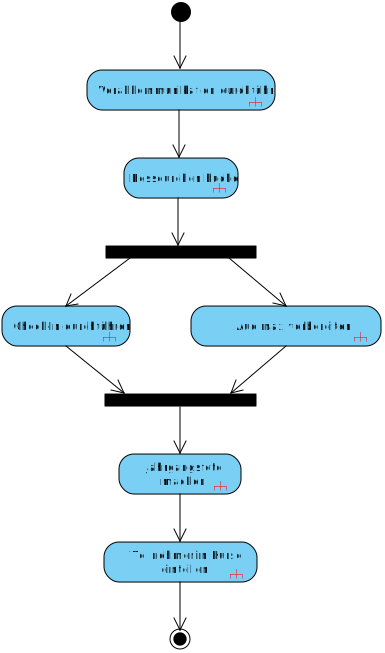
\includegraphics[width=0.3\columnwidth]{Bilder/act_Event_durchführen.pdf}
    \caption{Aktivitätsdiagramm zur Durchführung eines Events}
    \label{act:event-durchführen}
\end{figure}

\FloatBarrier

\subsection{Vorabkommunikation durchführen}
\autoref{act:vorabkomm-durchführen} zeigt die Aktivität \enquote{Vorabkommunikation durchführen}, in der im Vorfeld des Events alle notwendigen Informationen über das Event mittels E-Mail oder Telefon an die Teilnehmer übermittelt werden. Hierzu schreibt der Organisator zunächst eine entsprechende E-Mail und erstellt anschießend einen leeren Mailverteiler, welcher als Datastore modelliert wurde.

Als nächstes öffnet er den dem Event beigefügten Verweis mit allen Teilnehmern des Events. Sind noch nicht alle Teilnehmer des Events abgearbeitet, wird der nächste Teilnehmer des Events behandelt: Seine Kontaktdaten werden geöffnet, beinhalten diese eine E-Mail-Adresse, wird diese dem Mailverteiler hinzugefügt. Im ungünstigeren Fall ist für den Teilnehmer keine E-Mail-Adresse hinterlegt. In diesem Fall wird der Teilnehmer unter der in jedem Fall hinterlegten Telefonnummer angerufen. Nimmt der Teilnehmer den Anruf nicht an, wird dieser zur Liste der nicht erreichten Teilnehmer hinzugefügt. Nimmt der Teilnehmer das Gespräch an, fragt der Organisator ihn nach einer E-Mail-Adresse. Ist der Teilnehmer nicht gewillt oder nicht in der Lage dem Organisator eine E-Mail-Adresse zu nennen, warnt ihn der Organisator, dass so in Zukunft Informationen zu dem bevorstehenden Event nicht bei ihm ankommen könnten und übermittelt ihm die für das Event notwendigen Informationen telefonisch. Gibt der Teilnehmer am Telefon eine E-Mail-Adresse an, so wird diese dessen Kontaktdaten und dem Mailverteiler hinzugefügt. Diese beiden Aktionen laufen parallel ab. Dieser gesamte Vorgang wiederholt sich, bis alle Teilnehmer des Events abgearbeitet sind.

Es folgen nun zwei große Schleifen, welche parallel durchgeführt werden. In der linken Schleife wird versucht, die zuvor nicht erreichten Teilnehmer doch noch zu erreichen, um sie über alles nötige zu informieren. Hierzu wird zunächst die Liste der nicht erreichten Teilnehmer geöffnet. Sind noch nicht alle Teilnehmer abgearbeitet, wird der nächste Teilnehmer betrachtet, seine Kontaktdaten geöffnet und er unter der hinterlegten Telefonnummer angerufen. Nimmt dieser das Gespräch nicht an beginnt die Schleife mit dem nächsten Teilnehmer von neuem. Nimmt der Teilnehmer das Gespräch an, so wird er aus der Liste der nicht erreichten Teilnehmer entfernt und wie in der vorherigen Schleife nach einer E-Mail-Adresse gefragt. Ist der Teilnehmer nicht gewillt oder nicht in der Lage, dem Organisator eine E-Mail-Adresse zu nennen, warnt ihn der Organisator, dass so in Zukunft Informationen zu dem bevorstehenden Event nicht bei ihm ankommen könnten und übermittelt ihm die für das Event notwendigen Informationen telefonisch. Gibt der Teilnehmer am Telefon eine E-Mail-Adresse an, so wird diese dessen Kontaktdaten und dem Mailverteiler hinzugefügt. Diese beiden Aktionen laufen auch hier parallel ab. Dieser Vorgang wird für alle zuvor nicht erreichten Teilnehmer wiederholt, bis alle Teilnehmer die nötigen Informationen enthalten haben.

In der rechten Schleife, welche solange durchlaufen wird, bis das Event begonnen hat, werden zwei weitere Fehlerfälle behandelt, was ebenfalls parallel geschieht. Auf der linken Seite wird der Fall abgefangen, dass ein Teilnehmer absagt. Ist dieses der Fall, wird er aus der Liste der Teilnehmer des Events entfernt. Die rechte Seite zeigt, was geschehen soll, sollte das Event, beispielsweise aufgrund einer plötzlich auftretenden Pandemie, verboten werden. In diesem Fall wird der Status des Events auf \enquote{Abgesagt} gesetzt. Anschließend öffnet der Organisator die Ansprechpersonen des Events. Solange nicht alle Ansprechpersonen abgearbeitet sind, werden die Kontaktdaten des ersten Teilnehmers geöffnet, ist eine E-Mail-Adresse hinterlegt, wird eine E-Mail mit der Absage der Vor-Ort-Aktivitäten versendet. Ist keine E-Mail-Adresse vorhanden, wird der Teilnehmer telefonisch informiert. Nimmt er das Gespräch jedoch nicht an, wird der Teilnehmer auf die Liste der nicht erreichten Personen geschrieben. Dieses wiederholt sich solange, bis alle Teilnehmer einmal durchlaufen wurden. Anschließend werden die zuvor nicht erreichten Teilnehmer nach dem zuvor beschriebenen Prinzip über den Ausfall des Events informiert. Ist dies geschehen, so wird der Auftraggeber über die Notwendigkeit einer Alternative informiert. In diesem Fall wird die Aktion \enquote{Event durchführen} damit beendet.

Sind die beiden eben beschrieben Schleifen abgearbeitet, so wird der Status der Teileinheit \enquote{Vorabkommunikation} durchführen auf \enquote{Fertig} gesetzt.
\begin{figure}[ht!]
    \centering
    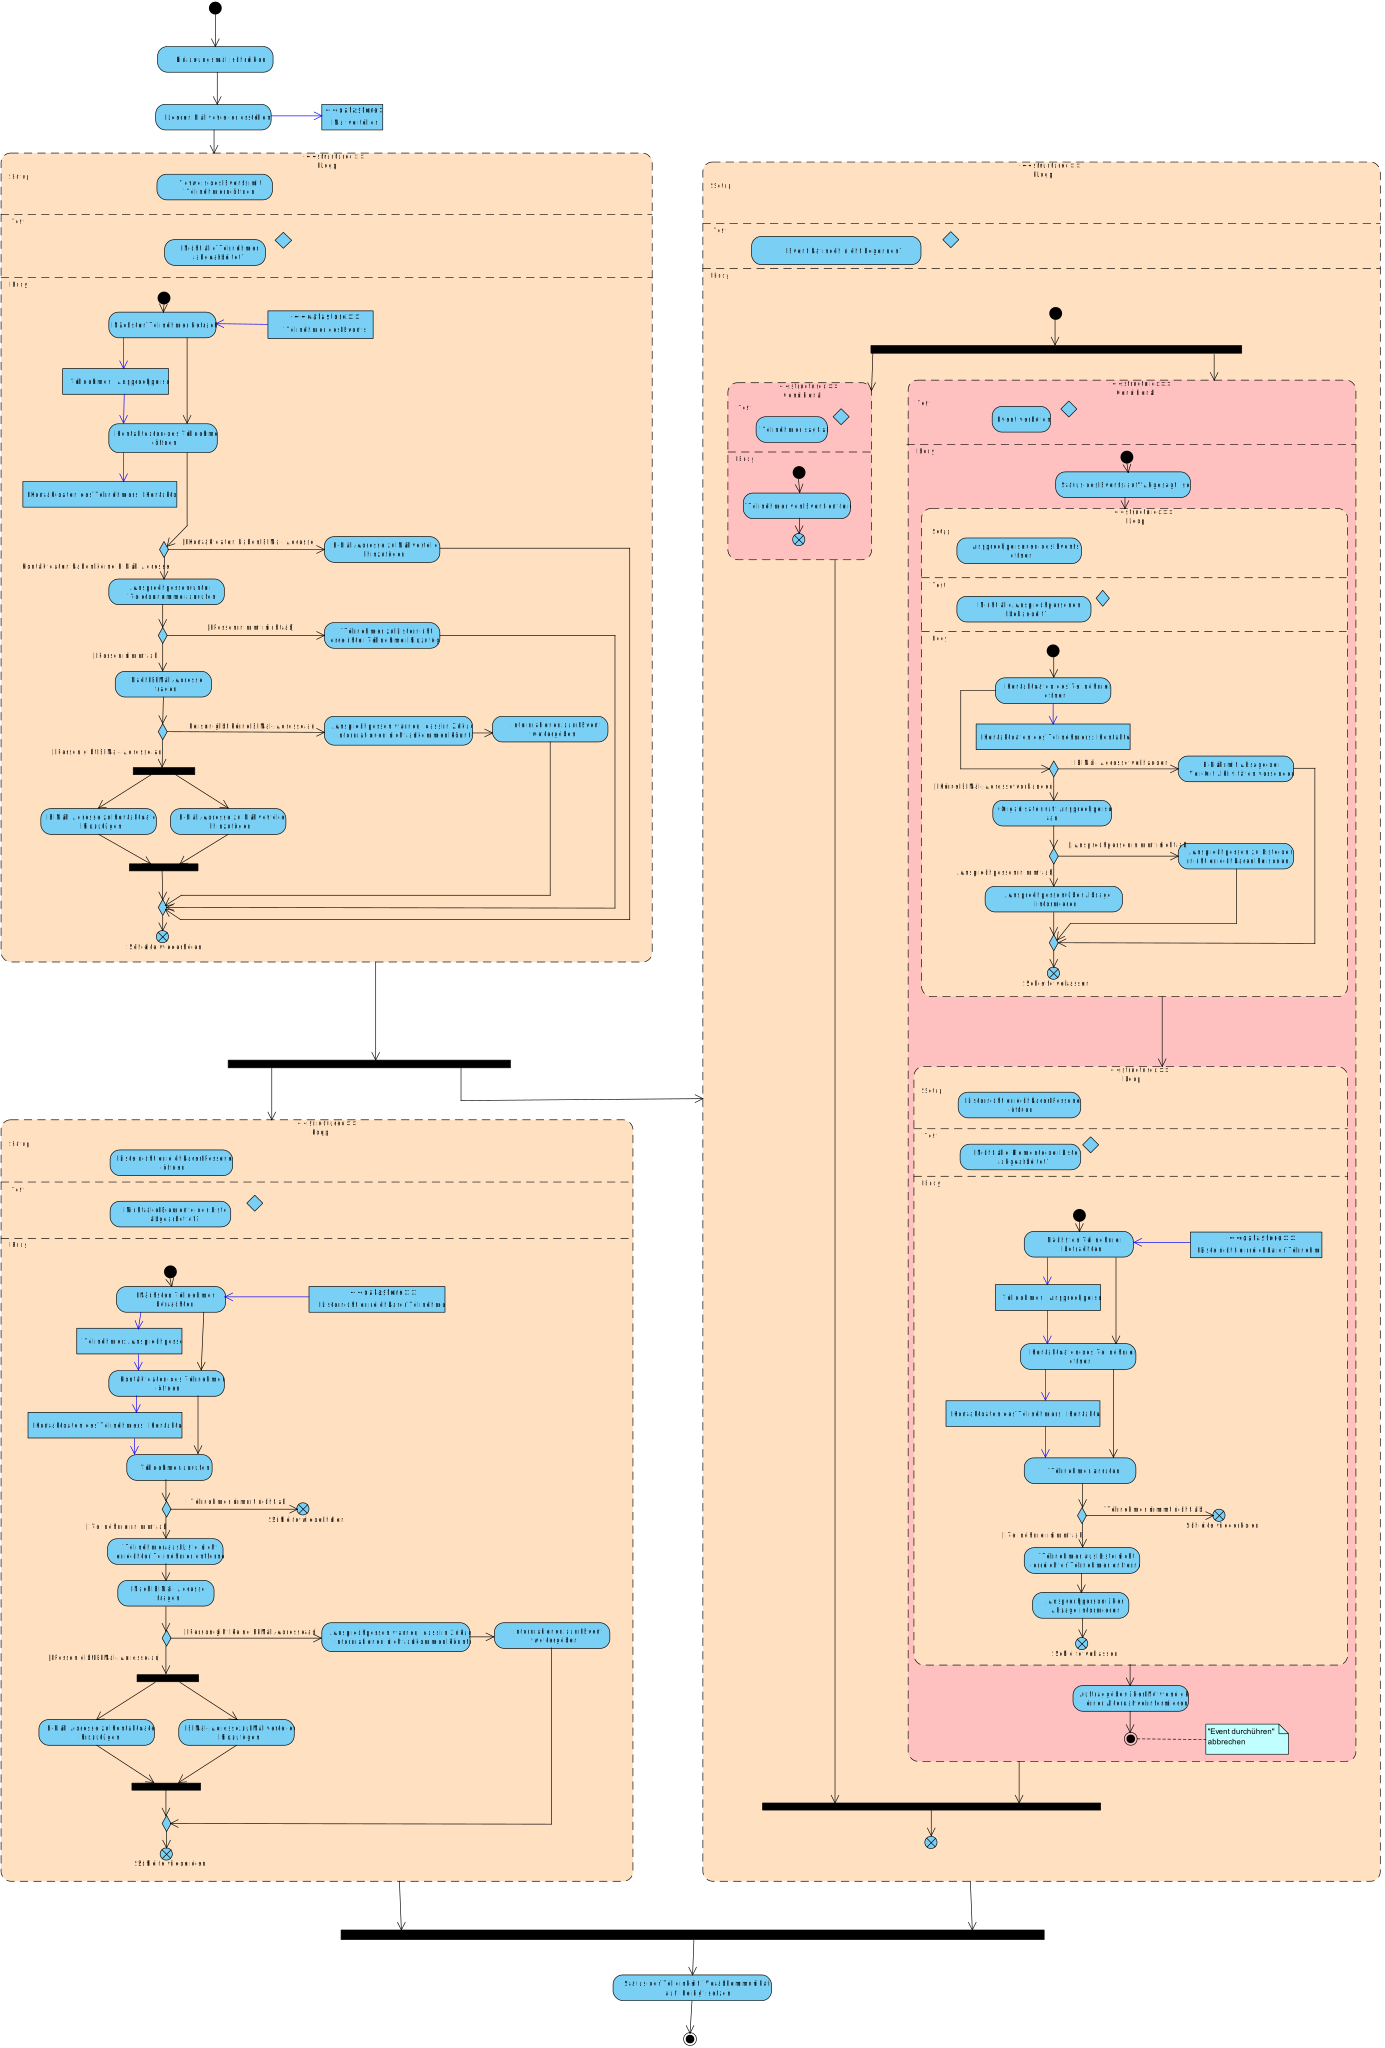
\includegraphics[width=0.65\columnwidth]{Bilder/act_Vorabkommunikation_durchführen.pdf}
    \caption{Aktivitätsdiagramm zur Durchführung der Vorabkommunikation}
    \label{act:vorabkomm-durchführen}
\end{figure}

\FloatBarrier

\subsection{Ressourcen buchen}
\autoref{act:ressourcen-buchen} zeigt die Aktivität \enquote{Ressourchen buchen}. Hier werden die für das Event notwendigen Lokationen und Personen gebucht. Hierbei handelt es sich um das Audimax, in dem alle neuen Studierenden Platz finden müssen, eine Wiese, auf der das Jahrgangsfoto aufgenommen werden soll sowie den dafür notwendigen Fotografen und schließlich um die Kursräume, in denen die Studierenden den restlichen Tag mit ihren Ausbildern verbringen.

\begin{figure}[ht!]
    \centering
    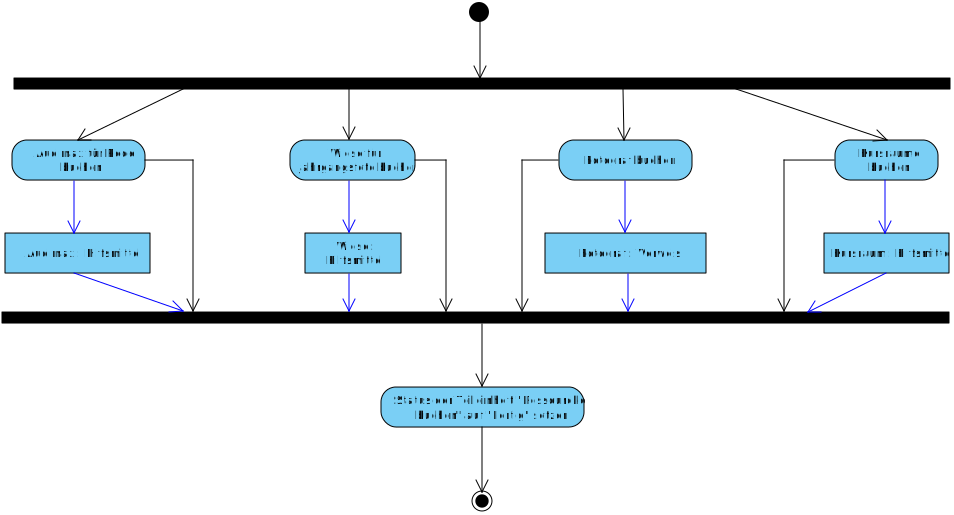
\includegraphics[width=0.8\columnwidth]{Bilder/act_Ressourcen_buchen.pdf}
    \caption{Aktivitätsdiagramm zum Ressourcen buchen}
    \label{act:ressourcen-buchen}
\end{figure}

Alle zuvor genannten Aktionen werden parallel ausgeführt. Sind sie alle abgeschlossen, wird der Status der zugehörigen Teileinheit \enquote{Ressourcen buchen} in den Status \enquote{Fertig} gesetzt.

\FloatBarrier

\subsection{Check-In durchführen}
\begin{figure}[ht!]
    \centering
    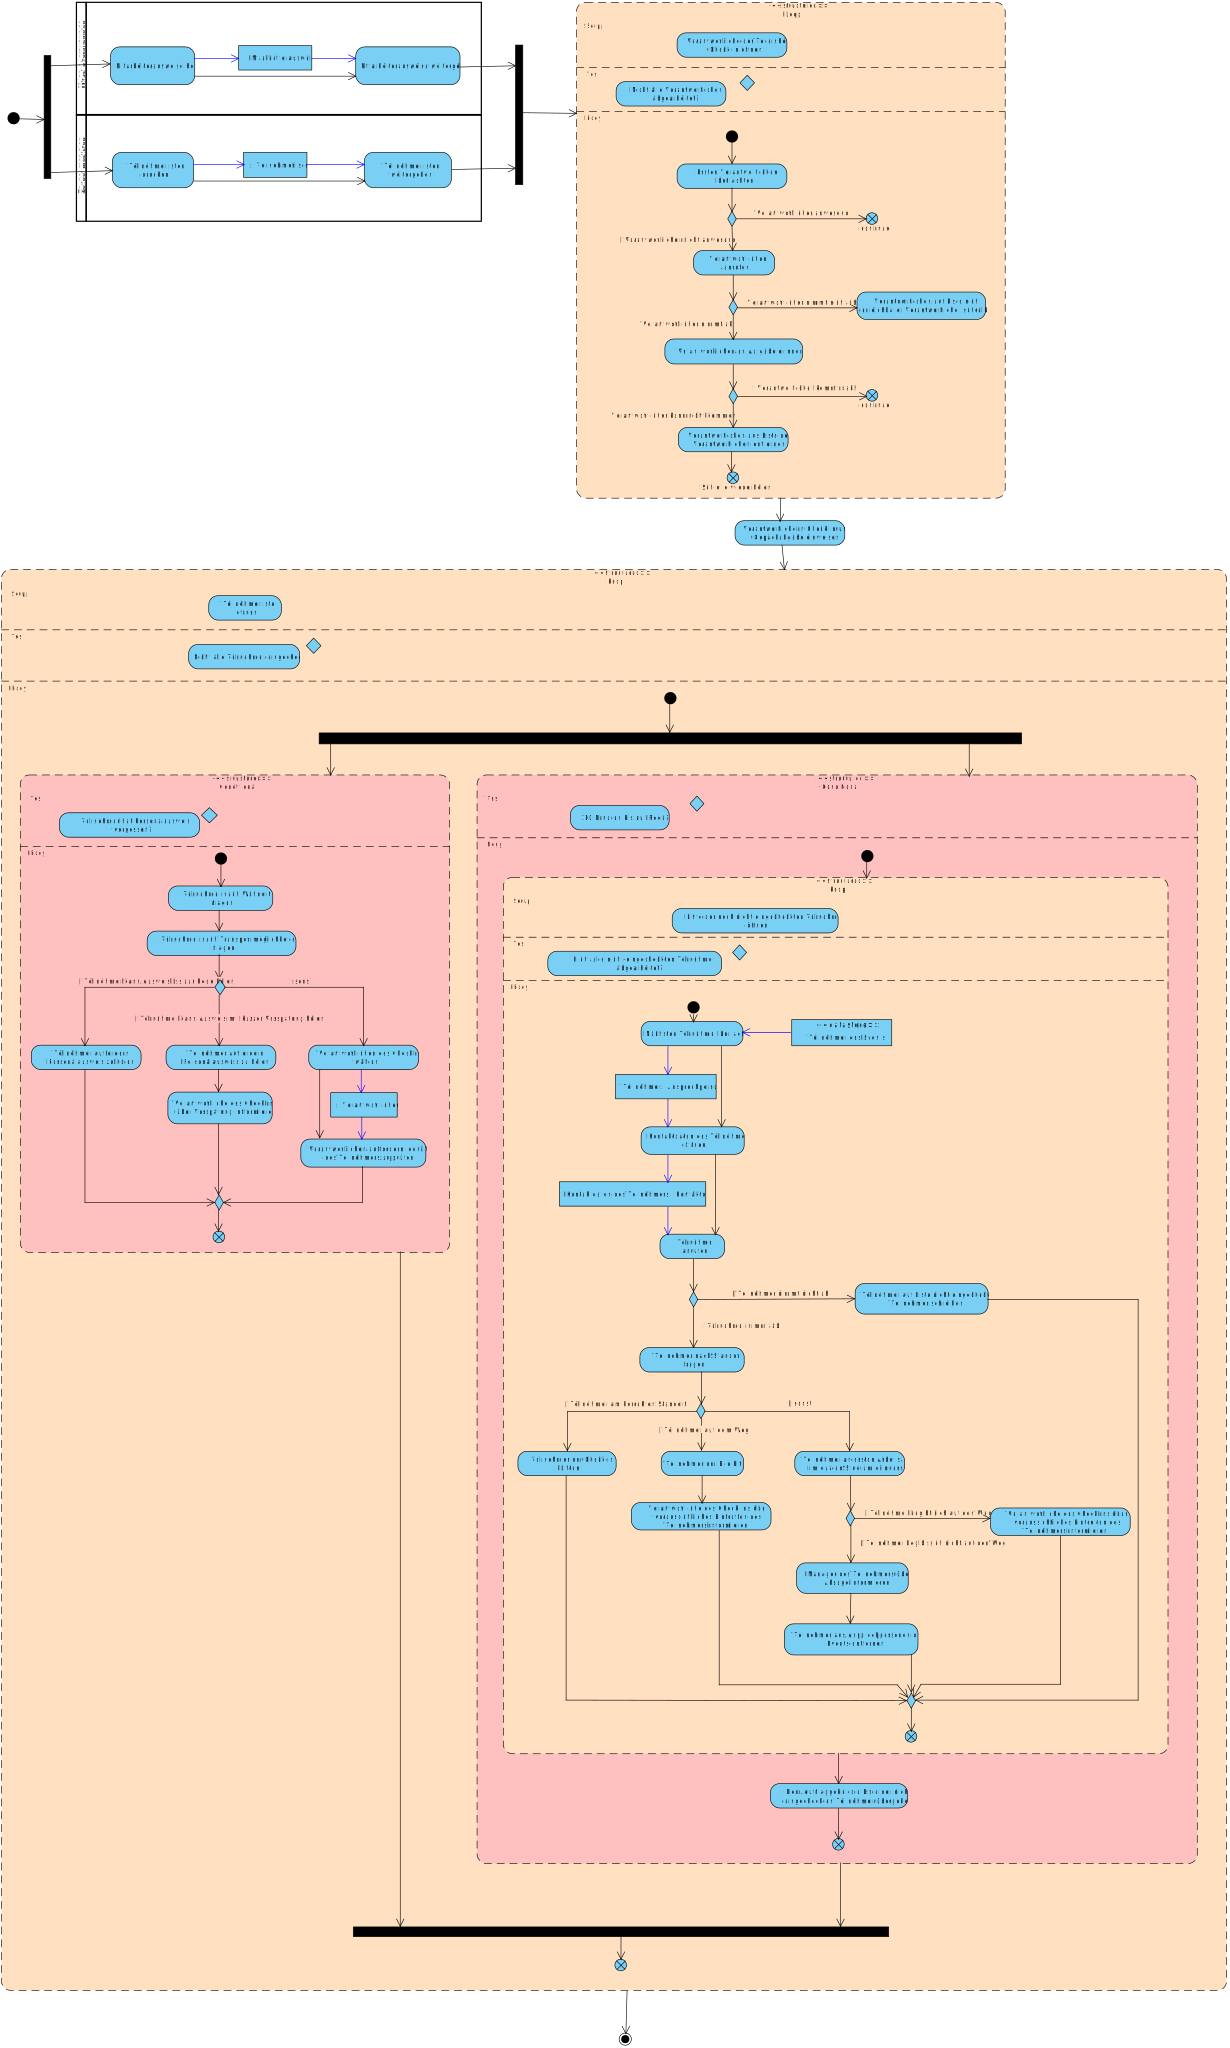
\includegraphics[width=0.7\columnwidth]{Bilder/act_Check_In.pdf}
    \caption{Aktivitätsdiagramm zur Durchführung des Check-Ins der Teilnehmer}
    \label{act:checkin-durchführen}
\end{figure}

Zu Beginn des Events werden alle Studenten begrüßt, ihr Eintreffen beim Check-In auf einer Liste festgehalten und ihnen wird ihr Mitarbeiterausweis ausgehändigt. Dafür ist es wichtig, dass jeder Student anhand seines Personalsausweises identifiziert wird, um nicht versehentlich der falschen Person einen Mitarbeiterausweis zu geben. Diese Vorgänge werden in \autoref{act:checkin-durchführen} dargestellt.

Um das zu erreichen, druckt der Organisator zuerst Teilnehmerlisten, anhand welcher später festgestellt wird, wer anwesend sein darf. Auch holt der Organisator die Mitarbeiterausweise beim Auftraggeber ab, welche an die Teilnehmer ausgeteilt werden.

Anschließend überprüft der Organisator die Anwesenheit aller eingeteilten Verantwortlichen für die Teileinheit des Check-Ins. Dafür öffnet er im Eventplanungssystem die Teileinheit Check-In und betrachtet die eingetragene Gruppe an Verantwortlichen. Ist ein Verantwortlicher nicht anwesend, so wird dieser angerufen. Kann ein Verantwortlicher dann nicht kommen, so wird dieser aus der Gruppe der zugewiesenen Verantwortlichen entfernt. Anschließend werden die anwesenden Verantwortlichen vom Organisator in ihre Check-In-Tätigkeit eingewiesen.

Während noch nicht alle Teilnehmer eingecheckt sind, hat der Organisator zwei verschiedene Fehlerfälle zu behandeln, sollten sie auftreten. Der erste ist dabei, dass ein Teilnehmer seinen Personalausweis vergisst. Sollte dieses auftreten, so wird wenn möglich der Teilnehmer nach Hause geschickt, um seinen Personalausweis zu besorgen. Sollte dieses nicht möglich sein, so sucht sich der Organisator einen Verantwortlichen aus, der damit beauftragt wird, den Teilnehmer als Einzelfall zu behandeln und auf andere Weise zu identifizieren.

Der andere Fall ist, falls zehn Minuten vor Beginn der Rede noch nicht alle Teilnehmer eingecheckt sind. Sollte dieses auftreten, so geht der Organisator die Liste der noch nicht eingecheckten Teilnehmer durch und ruft jeden einzelnen an. Nimmt ein Teilnehmer den Anruf nicht an, so wird dieser auf die Liste der nicht eingecheckten Teilnehmer geschrieben. Kann der Teilnehmer erreicht werden, so wird erfragt, ob dieser noch zum Event erscheinen wird. Ist dieses nicht der Fall, so wird der Teilnehmer ebenfalls auf die Liste gesetzt. Sind alle nicht eingecheckten Teilnehmer abgearbeitet, so leitet der Organisator die Liste mit den nicht eingecheckten Teilnehmern an den Auftraggeber weiter und informiert die zuständigen Manager über alle Absagen.

Nach dieser Fehlerbehandlung ist der Check-In vollständig abgearbeitet.

\subsection{Audimax vorbereiten}
\begin{figure}[ht!]
    \centering
    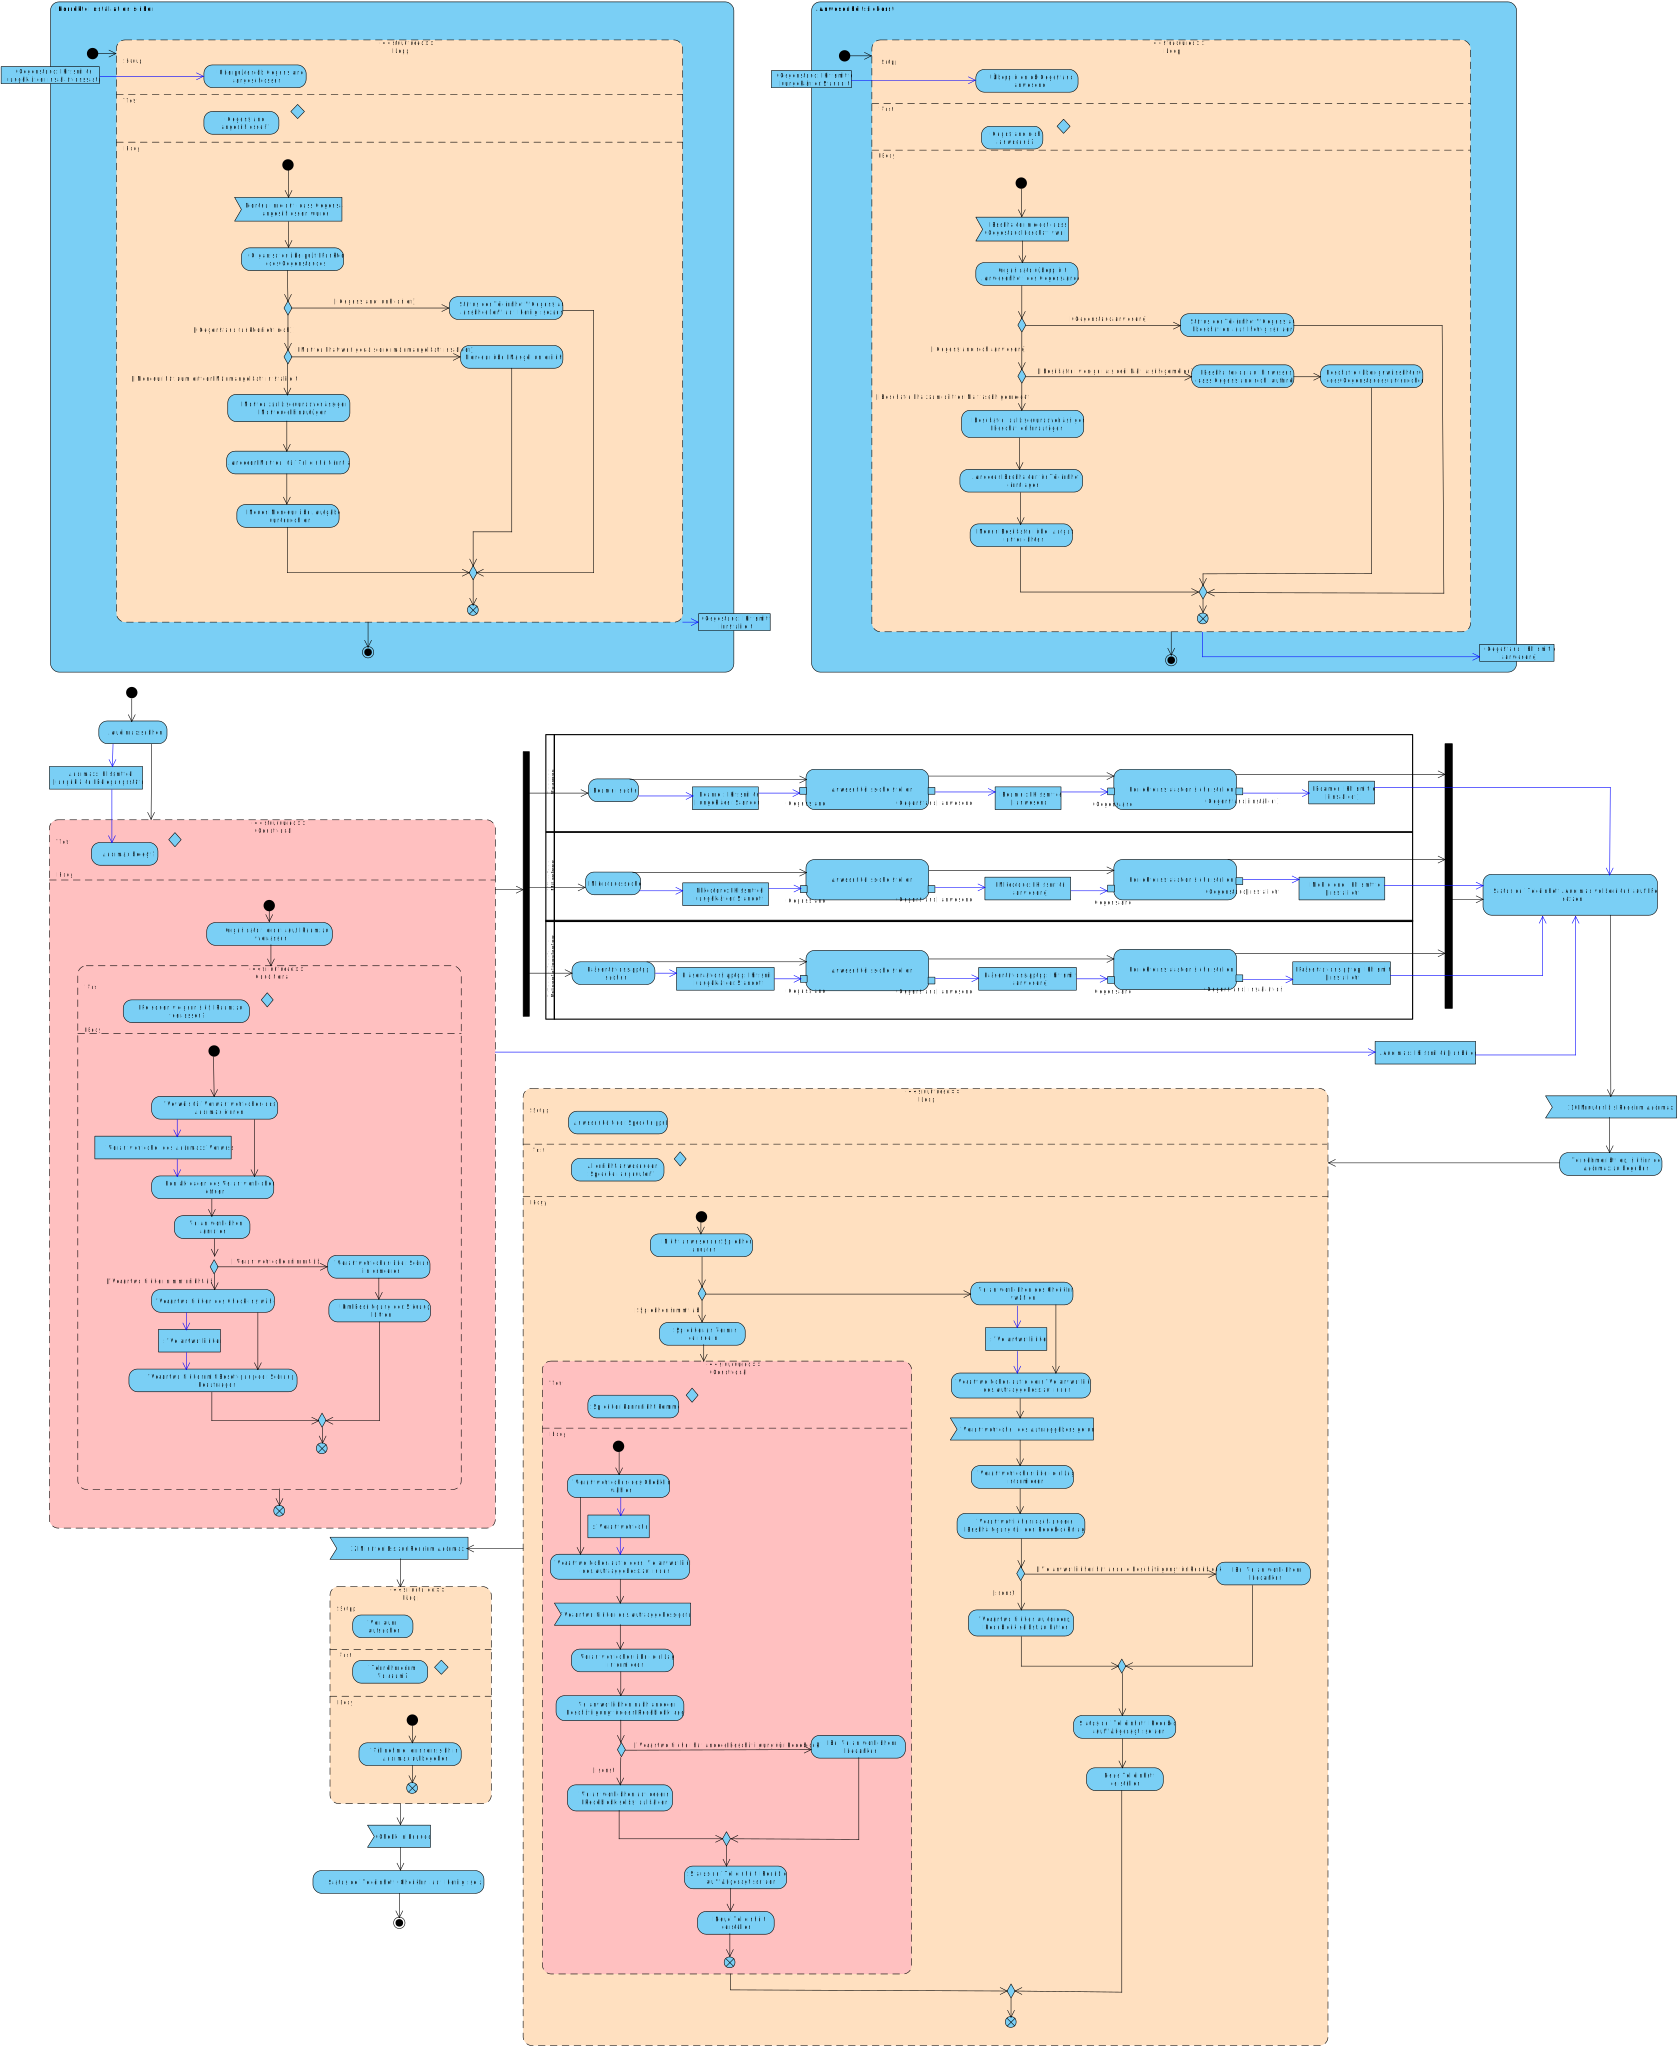
\includegraphics[width=0.7\columnwidth]{Bilder/act_Audimax_vorbereiten.pdf}
    \caption{Aktivitätsdiagramm zur Durchführung der Vorbereitung des Audimax}
    \label{act:audimax-vorbereiten}
\end{figure}

Um einen flüssigen Ablauf der Reden im Audimax zu sichern, werden parallel zum Check-In der Aufbau und die Vorbereitung des Audimax koordiniert. Dieser Vorgang wird in \autoref{act:audimax-vorbereiten} modelliert. Dafür sucht der Organisator den Raum auf, und prüft, ob dieser von anderen belegt ist. Sollte dieses der Fall sein, so fordert der Organisator die Störenden auf, den Raum zu verlassen. Sollte dieses nicht reichen, so ruft der Organisator den Verantwortlichen des Audimax an und fordert diesen auf, für eine Beseitigung der Störung zu sorgen. Sollte der Verantwortliche des Audimax nicht abnehmen, so beauftragt der Organisator einen Verantwortlichen des Check-Ins mit der Problemlösung. Es ist wichtig, dass der Organisator dieses delegiert, um im Falle eines Problems beim Check-In noch als Ansprechperson anwesend zu sein.

Nachdem dieses einen geräumten Raum bewirkt, werden die Beschaffer damit beauftragt, technisches Material zu beschaffen und am korrekten Ort zu platzieren. Um dieses zu modellieren, wurde links im Diagramm die Aktivität \code{Anwesenheit sicherstellen} allgemein definiert und wird hier in jeder Swimlane für den Beamer, die Mikrofone und den Präsentationslaptop genutzt. Die Aktivität hat einen Input-Pin und einen Output-Pin, welche definieren, dass ein Gegenstand ungeklärten Standortes hineingegeben und ein anwesender Gegenstand erhalten wird. Innerhalb der Aktivität wartet der Organisator darauf, dass der Beschaffer meldet, den Gegenstand beschafft zu haben. Sollte dieses passiert sein, so überprüft der Organisator die korrekte Anwesenheit und spricht Mängel an. Sollte ein Beschaffer die gleiche Aufgabe drei Mal hintereinander fälschlicherweise als gelöst melden, so wird ein anderer Beschaffer damit beauftragt, diese zu erledigen.

Nachdem sichergestellt ist, dass die Gegenstände anwesend sind, wird sichergestellt, dass sie auch korrekt installiert und funktionstüchtig sind. Dieser Prozess ist in der Aktivität \code{Korrekte Installation sicherstellen} modelliert und beschreibt einen ähnlichen Prozess zu dem des Sicherstellens der Anwesenheit eines Gegenstandes. Der Organisator prüft wieder die korrekte Installation und nennt dem Monteur aufgefallene Mängel. Ebenfalls hat jeder Monteur drei Versuche, bis ein anderer Monteur mit der Installation beauftragt wird. Dieses stellt sicher, dass sich kein Monteur zu lange an einer nicht für seine Kompetenzen geeigneten Aufgabe aufhält.

Nachdem so die korrekte Funktion von Beamer, Mikrofonen und Präsentationslaptop sichergestellt ist, kann der Organisator die Teileinheit \enquote{Audimax vorbereiten} in den Status \enquote{Fertig} setzen. Dann ist keine weitere Tätigkeit bis zehn Minuten vor den Reden nötig. Erst dann werden die Teilnehmer in das Audimax gebeten und der Organisator überprüft die Anwesenheit aller eingeladenen Sprecher. Sollte ein Sprecher nicht anwesend sein, so wird dieser angerufen. Sollte der Sprecher das Telefongespräch annehmen und rechtzeitig kommen können, so wird einfach weiter verfahren, andernfalls wird ein Verantwortlicher des Auftraggebers gefunden, der mit der Problemlösung beauftragt wird. 

Abschließend werden zwei Minuten vor Beginn der Reden die letzten Teilnehmer aus dem Vorraum ins Audimax gebeten. Ist der Check-In beendet, so wird die Teileinheit \enquote{Check-In} in den Status \enquote{Fertig} gesetzt.

\subsection{Neue Teileinheit erstellen}
In \autoref{act:teileinheit-erstellen} wird die Aktivität \enquote{Teileinheitt erstellen} modelliert, welche im Zuge einer schnellen Umplanung verwendet wird. Es wird zunächst eine neue Teileinheit erstellt, wobei ein initiales Teileinheittobjekt entsteht. Dieses durchläuft mit dem Objectflow alle nachfolgenden Aktionen der Aktivität. Die nächste ist das Hinzufügen eines Verweises auf den Auftraggeber des Events, um dessen Kontaktdaten stets schnell parat zu haben. Dann wird in der Beschreibung der Teileinheit eine Beschreibung der mit der Teileinheit neu geplanten Alternativtätigkeit angegeben. Anschließend wird ein Verantwortlicher für die Teileinheit hinzugefügt und abschließend werden die Voraussetzungen für die Teileinheit festgelegt.

\begin{figure}[ht!]
    \centering
    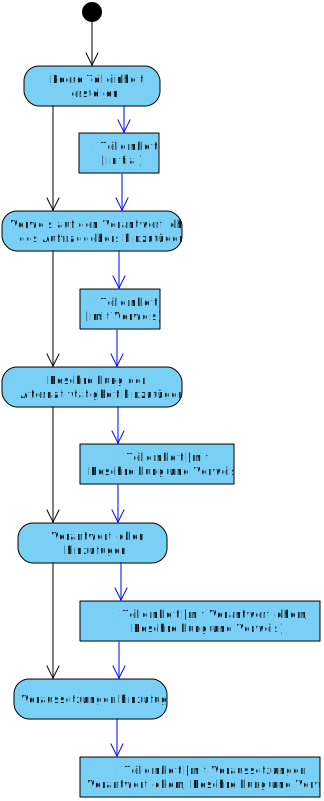
\includegraphics[width=0.3\columnwidth]{Bilder/act_Neues_Teilevent_erstellen.pdf}
    \caption{Aktivitätsdiagramm zum Erstellen einer Teileinheit}
    \label{act:teileinheit-erstellen}
\end{figure}

\FloatBarrier

\subsection{Jahrgangsfoto machen}
Die in \autoref{act:jahrgangsfoto-machen} modellierte Aktivität \enquote{Jahrgangsfoto machen} beginnt sobald die im Audimax gehaltenen Reden noch 10 Minuten dauern. Dies wurde mittels eines Ereignisempfängers dargestellt. 

Es wird zunächst der Fall behandelt, dass der Fotograf noch nicht eingetroffen ist. In diesem Fall öffnet der Organisator zunächst den Verweis auf den Fotografen in der Teileinheit \enquote{Jahrgangsfoto machen}, öffnet dessen beigefügte Kontaktdaten und ruft diesen auf der in den Kontaktdaten hinterlegten Telefonnummer an. Für den Fall, dass der Fotograf den Anruf nicht annimmt, wählt der Organisator einen Verantwortlichen des Check-Ins aus und beauftragt diesen, eine Alternative zu dem ausgefallenen Fotografen ausfindig zu machen. Nimmt der Fotograf das Telefongespräch an, fragt der Organisator diesen nach seinem Standort. Nun werden drei Fälle unterschieden: Entweder der Fotograf ist bereits auf dem Weg, dann bittet der Organisator ihn lediglich um Eile, oder der Fotograf ist verhindert. Auch in diesem Fall wählt der Organisator einen Verantwortlichen des Check-Ins aus, um diesen zu beauftragen, eine Alternative zu dem Fotografen ausfindig zu machen. In allen anderen Fällen bittet der Organisator den Fotografen, rechtzeitig zu kommen. Damit ist der Fehlerfall vollständig behandelt.

Die folgenden Aktionen beginnen, sobald der Fotograf eintrifft. Diesem zeigt der Organisator zunächst die Wiese, auf der das Jahrgangsfoto aufgenommen werden soll und erklärt ihm die Anforderungen an das Foto. Sind die Reden im Audimax beendet, wird dann der Status der Teileinheit \enquote{Reden} auf \enquote{Fertig} gesetzt. Anschließend werden die Teilnehmer daüber informiert, dass nun das Jahrgangsfoto aufgenommen wird, dass dieses freiwillig ist und zuvor ein Datenschutzhinweis unterschrieben werden muss. Ist dies geschehen, werden die Teilnehmer angewiesen, sich auf die Wiese zu begeben. 

In der nachfolgenden Schleife wird sichergestellt, dass alle Teilnehmer, welche auf das Jahrgangsfoto möchten, sich aus dem Audimax auf die Wiese begeben haben. Hierzu sucht der Organisator zunächst das Audimax auf, überprüft, ob sich noch noch Teilnehmer im Audimax aufhalten. Ist dies der Fall, weist der Organisator sie an, sich auf die Wiese zu begeben.

Als nächstes wird von jedem der Teilnehmer des Jahrgangsfotos die Unterschrift der Datenschutzerklärung gefordert. Ist das Jahrgangsfoto gemacht, wird der Status der entsprechenden Teileinheit auf \enquote{Fertig} gesetzt und der Fotograf verabschiedet. Damit ist die die Aktivität \enquote{Jahrgangsfoto machen} abgeschlossen.
\begin{figure}[ht!]
    \centering
    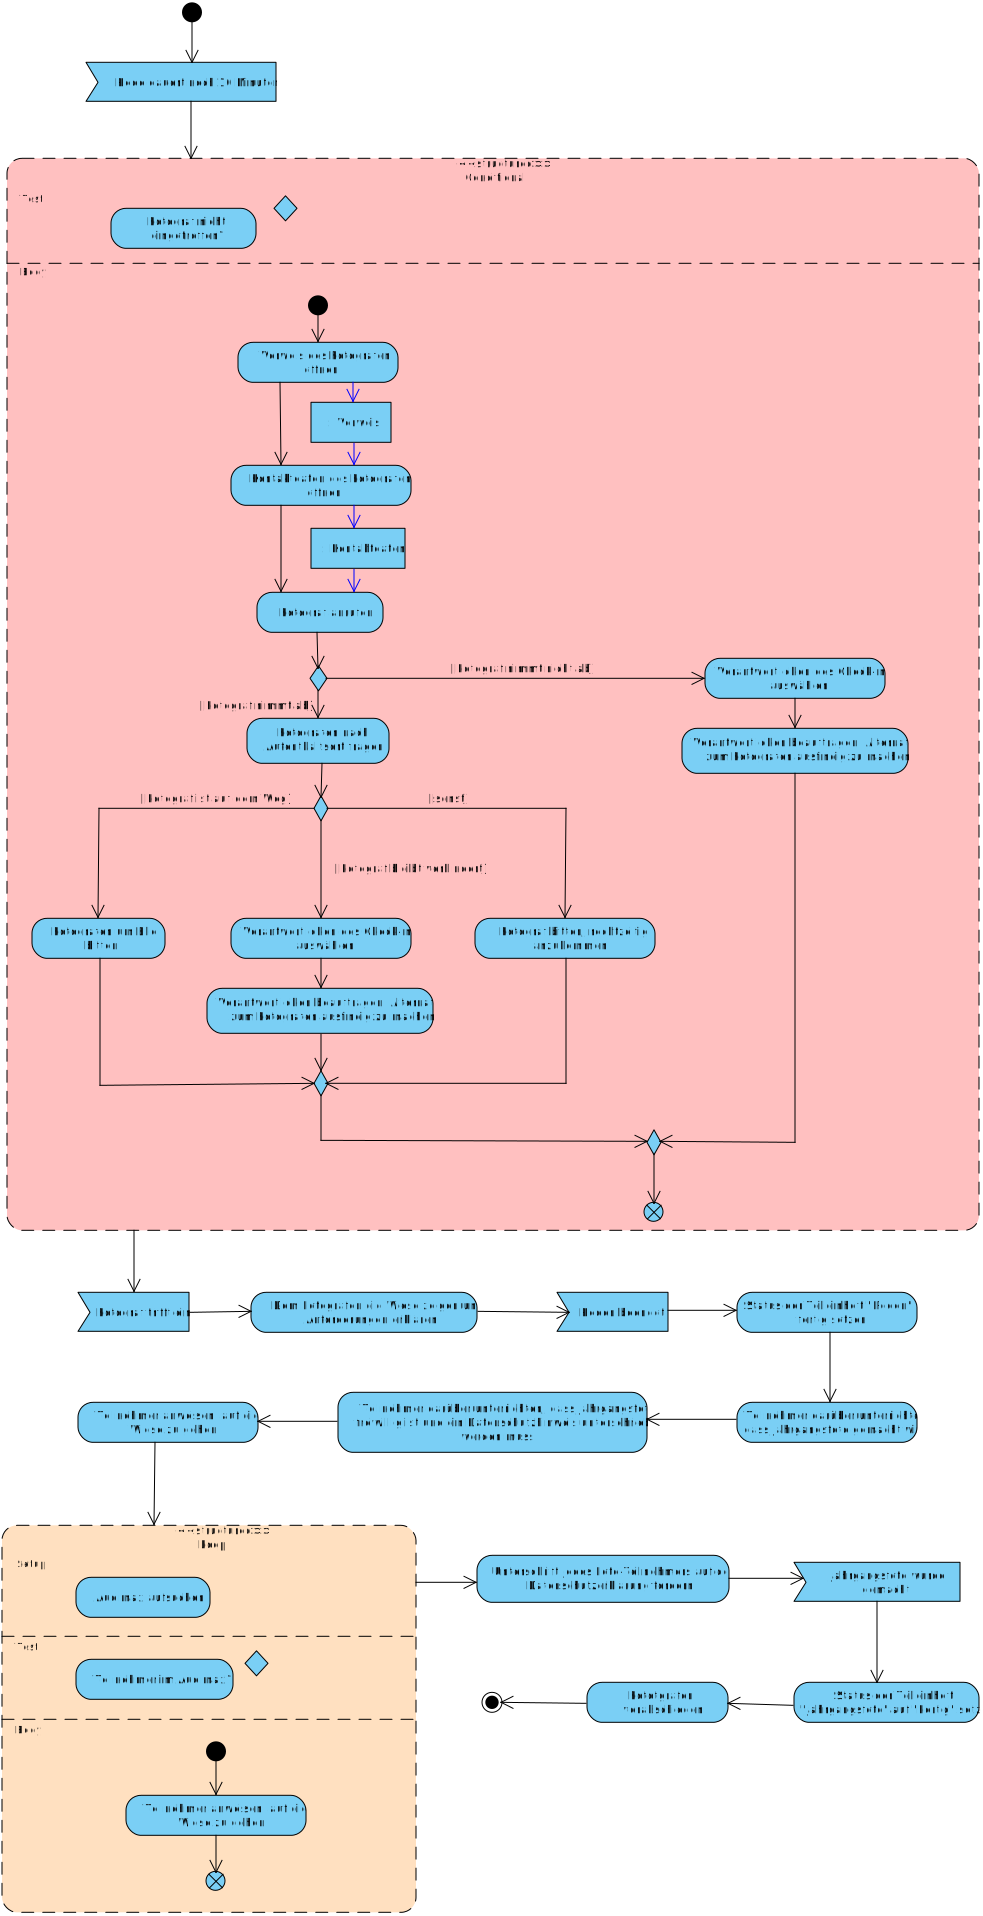
\includegraphics[width=0.6\columnwidth]{Bilder/act_Jahrgangsfoto_machen.pdf}
    \caption{Aktivitätsdiagramm zur Erstellung des Jahrgangsfotos}
    \label{act:jahrgangsfoto-machen}
\end{figure}

\FloatBarrier

\subsection{Teilnehmer in Kurse einteilen}
\begin{figure}[ht!]
    \centering
    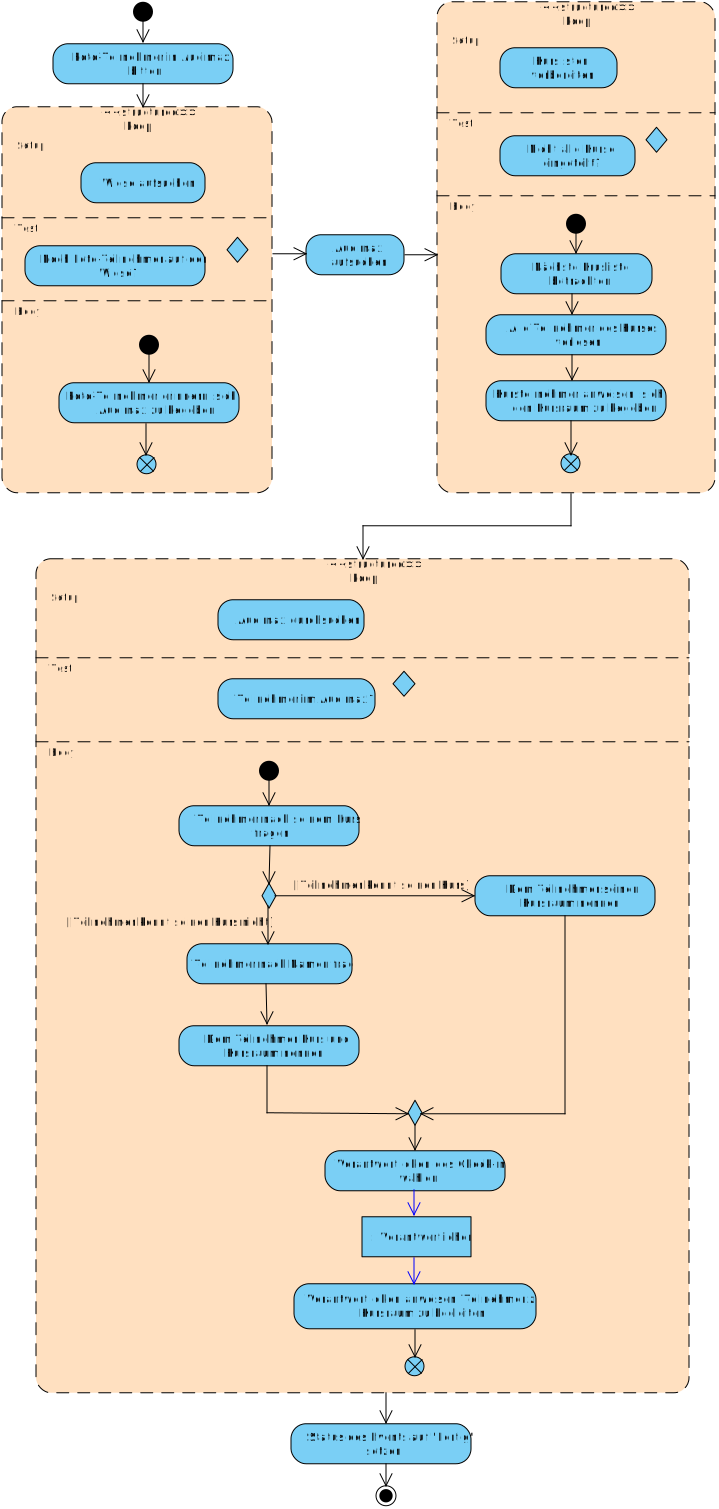
\includegraphics[width=0.7\columnwidth]{Bilder/act_Teilnehmer_in_Kurse_einteilen.pdf}
    \caption{Aktivitätsdiagramm zur Durchführung der Aufteilung der Teilnehmer in ihre Kurse}
    \label{act:teilnehmer-einteilen}
\end{figure}

\autoref{act:teilnehmer-einteilen} visualisiert das Einteilen der Teilnehmer in ihre Kurse. Hierzu werden zuerst die Foto-Teilnehmer wieder in das Audimax gebeten und solange sich noch Teilnehmer auf der Wiese befinden, diese wiederholt daran erinnert, sich wieder in das Audimax zu begeben. Im Audimax wird anschließend für jeden Kurs eine Liste aller Teilnehmer vorgelesen und der zugehörige Kursraum. Die entsprechenden Teilnehmer gehen dann mit ihrem Ausbilder in den Kursraum. Sollten nach Abarbeiten aller Kurse noch Teilnehmer im Audimax sein, so werden diese einzeln abgearbeitet. Dafür werden sie zuerst nach ihrem Kurs gefragt und falls sie diesen nicht kennen nach ihrem Namen. Anschließend wird ihnen der entsprechende Kursraum genannt und sie werden von einem Verantwortlichen des Check-Ins zu diesem gebracht.

Als letzte Aktion des Tages setzt der Organisator das Event in den Status \enquote{Fertig}.
